\documentclass[journal,12pt,onecolumn]{IEEEtran}
\usepackage{cite}
\usepackage{caption}
\usepackage{graphicx}
\usepackage{amsmath,amssymb,amsfonts,amsthm}
\usepackage{algorithmic}
\usepackage{graphicx}
\usepackage{textcomp}
\usepackage{xcolor}
\usepackage{tfrupee}
\usepackage{txfonts}
\usepackage{listings}
\usepackage{enumitem}
\usepackage{mathtools}
\usepackage{gensymb}
\usepackage{comment}
\usepackage[breaklinks=true]{hyperref}
\usepackage{tkz-euclide} 
\usepackage{listings}
\usepackage{gvv}
%\def\inputGnumericTable{}
\usepackage[latin1]{inputenc} 
\usetikzlibrary{arrows.meta, positioning}
\usepackage{xparse}
\usepackage{color}                                            
\usepackage{array}                                            
\usepackage{longtable}                                       
\usepackage{calc}                                             
\usepackage{multirow}
\usepackage{multicol}
\usepackage{hhline}                                           
\usepackage{ifthen}                                           
\usepackage{lscape}
\usepackage{tabularx}
\usepackage{array}
\usepackage{float}
\usepackage{marvosym}
\usepackage{float}
%\newcommand{\define}{\stackrel{\triangle}{=}}
\theoremstyle{remark}
\usepackage{circuitikz}
\captionsetup{justification=centering}
\usepackage{tikz}

\title{Matrices in Geometry 9.5.1}
\author{EE25BTECH11037 - Divyansh}
\begin{document}
\vspace{3cm}
\maketitle
{\let\newpage\relax\maketitle}
\textbf{Question: }
Find the roots of 
\begin{align}
    x^2 + 3x -10=0
\end{align}
\vspace{2mm}


\textbf{Solution:}
Expressing the given equation as parabola 
\begin{align}
    y=x^2 + 3x -10
\end{align}
Representing this equation as a conic section
\begin{align}
    \vec{x}^{\top}\vec{V}\vec{x} + 2\vec{u}^{\top}\vec{x} + f=0 \ , \  \vec{V}=\myvec{1 & 0\\0&0} \ , \  \vec{u}=\myvec{3/2 \\ -1/2} \ ,\ f=-10
\end{align}
We need to find intersection points with $y=0$, that is, the X-axis.
\begin{align}
    \vec{x}=\vec{h} + k \vec{m} \ , \ \vec{h}=\myvec{0 \\ 0} \ , \ \vec{m}=\myvec{1 \\ 0}
\end{align}
Substituting $\vec{x} = k \vec{m}$ 
\begin{align}
    k^2\vec{m}^{\top}\vec{V}\vec{m} + 2k\vec{u}^{\top}\vec{m} + f=0 \\
    \implies k= \dfrac{1}{2} \sbrak{ -2\vec{u}^{\top}\vec{m} \ \pm \ \sqrt{4\brak{\vec{u}^{\top}\vec{m}}^2 - 4 f \vec{m}^{\top}\vec{V}\vec{m}}}\\
    \implies k= -\vec{u}^{\top}\vec{m} \ \pm \ \sqrt{\brak{\vec{u}^{\top}\vec{m}}^2-f \vec{m}^{\top}\vec{V}\vec{m}}\\
    \vec{u}^{\top}\vec{m} = \myvec{3/2 & -1/2}\myvec{1 \\0} =3/2 \\
    \vec{m}^{\top}\vec{V}\vec{m}=\myvec{1 & 0}\myvec{1 & 0\\0&0}\myvec{1 \\ 0} = 1\\
    k= -\dfrac{3}{2} \ \pm \ \sqrt{ \dfrac{9}{4 } - \brak{-10} 1} = -\dfrac{3}{2} \ \pm \sqrt{\dfrac{49}{4}}\\
    \implies k= - \dfrac{3}{2} \ \pm \dfrac{7}{2}\implies \boxed{ k= 2 \text{ OR } k=-5}
\end{align}
Substituting $k$ into $\vec{x}$, we get
\begin{align}
    \vec{x} = \myvec{2 \\ 0} \text{ OR } \vec{x}=\myvec{-5 \\ 0}
\end{align}
This implies that the roots of $x^2 +3x -10 =0$ are $2$ and $-5$.\\
Let us plot this
\begin{figure}
    \centering
    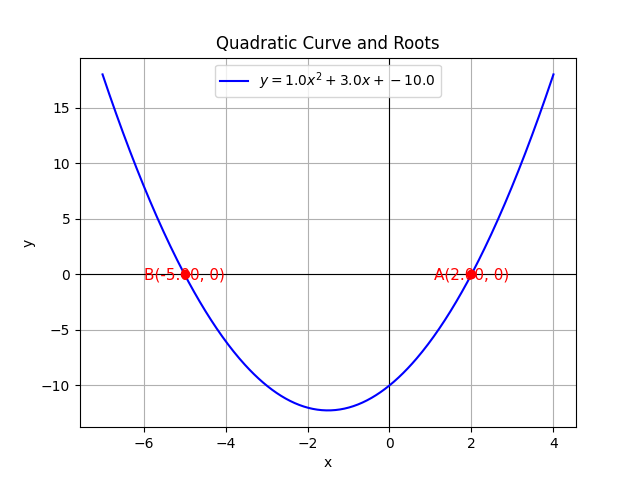
\includegraphics[width=1\columnwidth]{figs/1.png}
    \caption{Graph for 9.5.1}
    \label{fig:placeholder}
\end{figure}
\end{document}


